% \textbf{\underline{OZ 5 - Magnetische inductie en de wet van Faraday - Oefening 1:}}
% \vspace{0.5cm}

% Door een solenoïde met straal $ r = 1,25 $ cm, lengte $ l = 30,00 $ cm, en 300 wikkelingen loopt een stroom van 12,0 A.

% \begin{enumerate}[(a)]
%     \item Bereken de magnetische flux door een schijfvormig oppervlak met straal $ R = 5,00 $ cm dat loodrecht op en in het midden van de as van de solenoïde staat (Figuur 5.1a).
%     \item Doe nu hetzelfde voor het ringvormige oppervlak in Figuur 5.1b met $ a = 0,400 $ cm en $ b = 0,800 $ cm. 
% \end{enumerate}

% \begin{figure}[H]
%     \centering
%     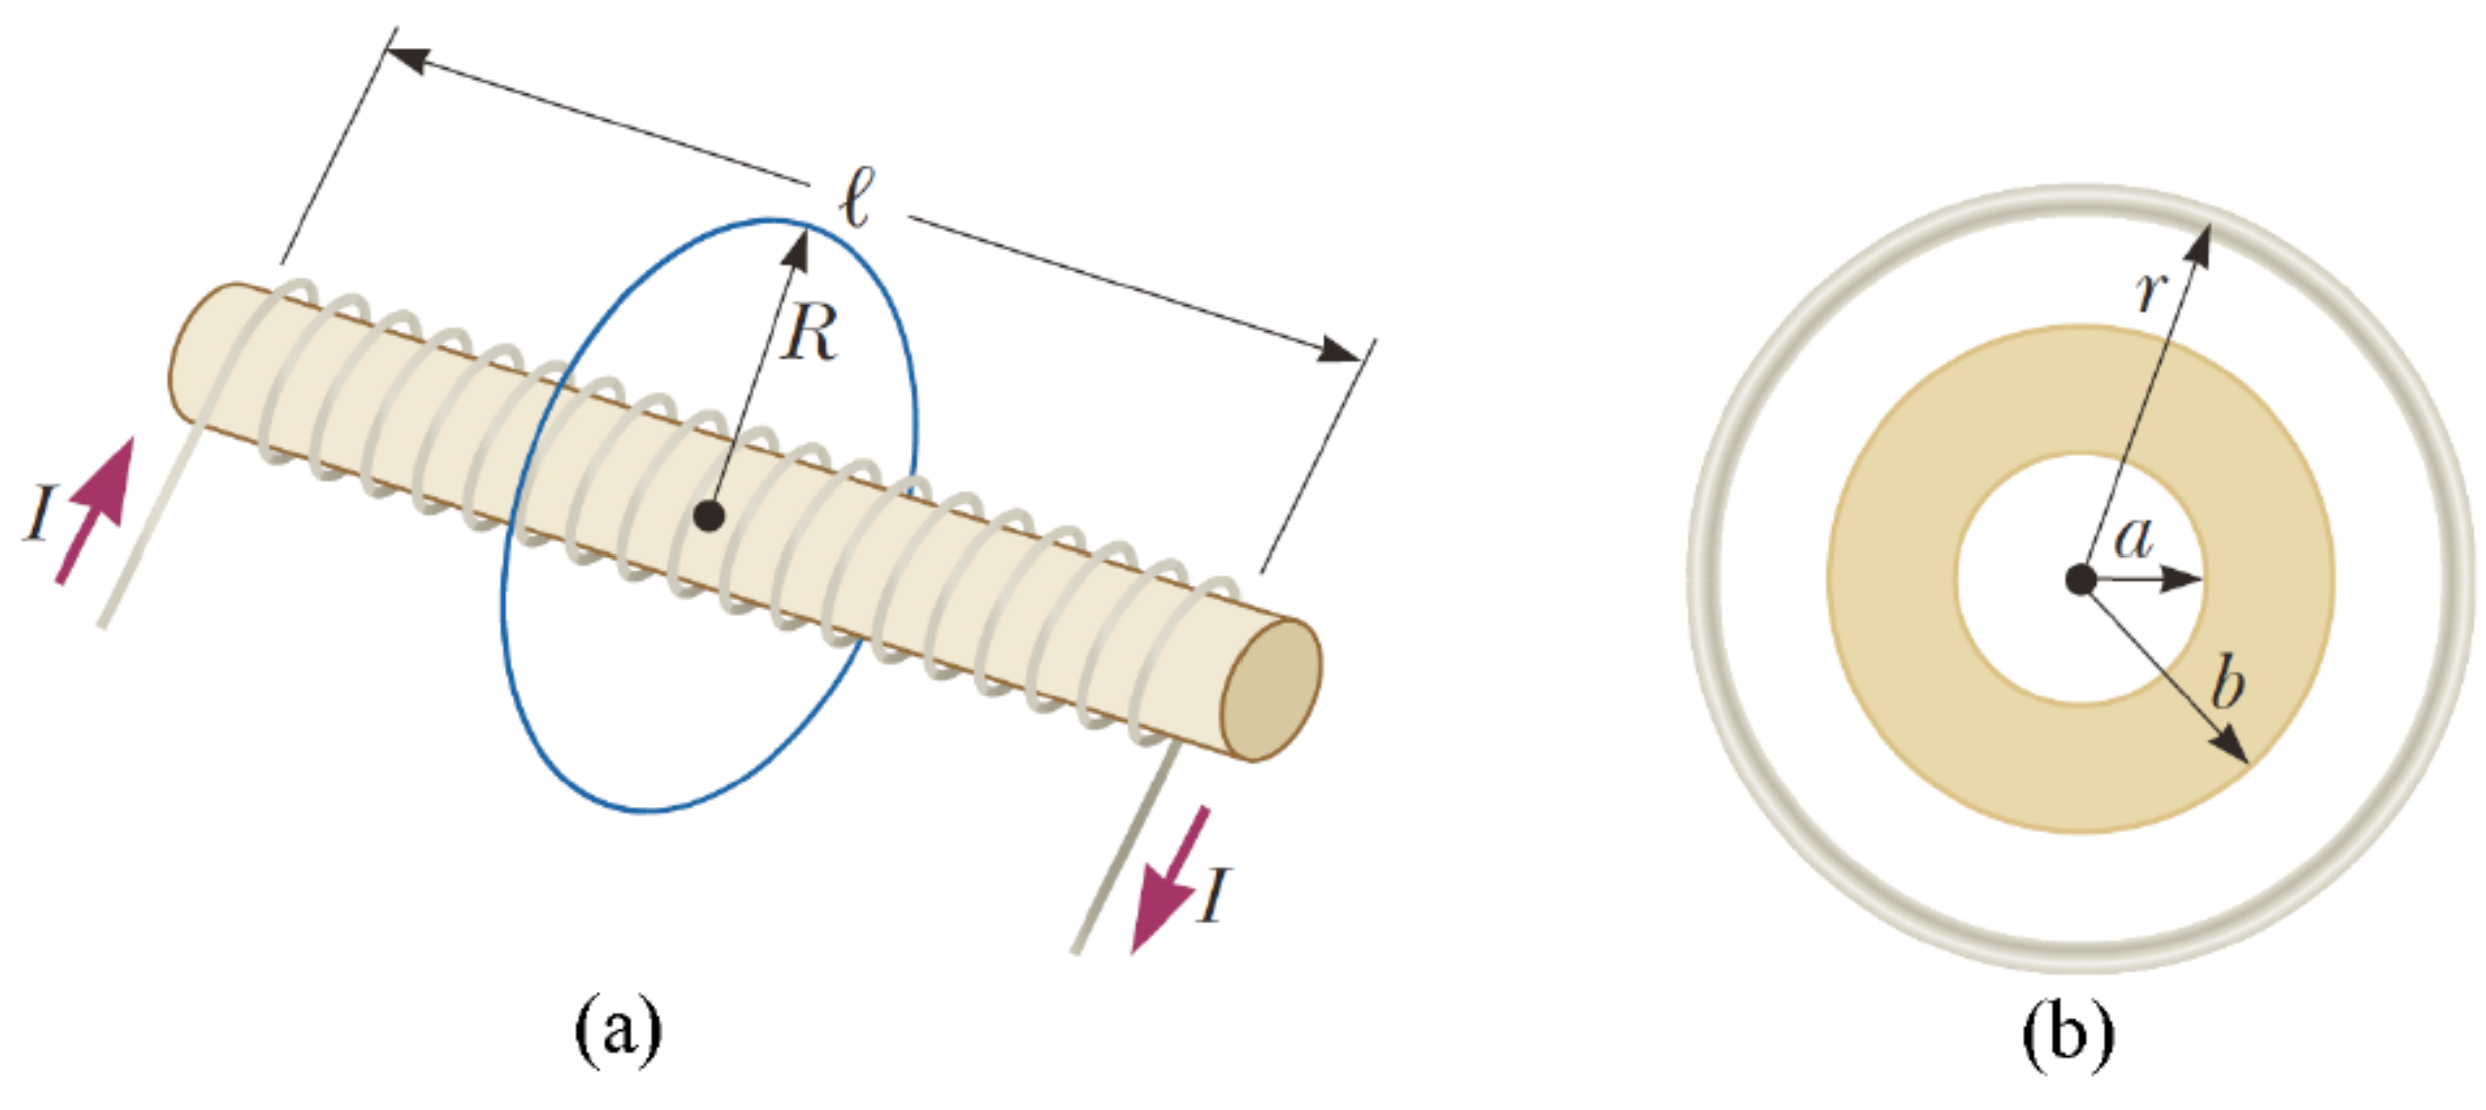
\includegraphics[width=8cm]{oz05/resources/oef-1-opgave.png}
    
%     \textbf{Figuur 5.1}
% \end{figure}

% \begin{description}[labelwidth=1.5cm, leftmargin=!]
%     \item[Geg. :]   $ r = 1,25 $ cm; $ l = 30,00 $ cm; $ N = 300 $; $ I = 12,0 $ A;
% \end{description}

% \begin{enumerate}[(a)]
%     \item 
%         \begin{description}[labelwidth=1.5cm, leftmargin=!]
%             \item[Geg. :]   $ R = 5,00 $ cm;
%             \item[Gevr. :]  $ \Phi_B $;
%             \item[Opl. :]   $ B = \dfrac{\mu_0 N I}{l} = \dfrac{4\pi \cdot 10^{-7} \cdot 300 \cdot 12,0}{30,00 \cdot 10^{-2}} = \dfrac{3\pi}{625} $ T
            
%                             \vspace{0.5cm}
                            
%                             $ A = \pi r^2 = \pi \cdot \left( 1,250 \cdot 10^{-2} \right)^2 = 0,00015625\pi $ m$ ^2 $
                            
%                             $ \Phi_B = \int \vec{B} \cdot  d\vec{A} = B \cdot A = \dfrac{3\pi}{625} \cdot 0,00015625\pi = 0,000007402 \textrm{ Wb} \approx 7,40 \ \mu $Wb
%         \end{description}
%     \item
%         \begin{description}[labelwidth=1.5cm, leftmargin=!]
%             \item[Geg. :]   $ a = 0,400 $ cm; $ b = 0,800 $ cm;
%             \item[Gevr. :]  $ \Phi_B $;
%             \item[Opl. :]   $ B = \dfrac{\mu_0 N I}{l} = \dfrac{4\pi \cdot 10^{-7} \cdot 300 \cdot 12,0}{30,00 \cdot 10^{-2}} = \dfrac{3\pi}{625} $ T
            
%                             \vspace{0.5cm}
                            
%                             $ A = \pi b^2 - \pi a^2 = \pi \cdot \left( 0,800 \cdot 10^{-2} \right)^2 - \pi \cdot \left( 0,400 \cdot 10^{-2} \right)^2 = 0,000048\pi $ m$ ^2 $
            
%                             \vspace{0.5cm}
                            
%                             $ \Phi_B = \int \vec{B} \cdot d\vec{A} = B \cdot A = \dfrac{3\pi}{625} \cdot 0,000048\pi = 0,000002274 \textrm{ Wb} \approx 2,27 \ \mu $Wb
%         \end{description}
% \end{enumerate}

% \vspace{1cm}